\documentclass[conf]{new-aiaa}
%\documentclass[journal]{new-aiaa} for journal papers
\usepackage[utf8]{inputenc}

\usepackage{graphicx}
\usepackage{amsmath}
\usepackage[makeroom]{cancel}
\usepackage[version=4]{mhchem}
\usepackage{siunitx}
\usepackage{longtable,tabularx}
\usepackage[framed,numbered,autolinebreaks,useliterate]{mcode}
\setlength\LTleft{0pt} 
\usepackage{gensymb}
\usepackage{rotating}
\usepackage{hyperref}
\title{ME509 Heat Transfer Final Exam}

\author{Tobin A. Nelson}
\affil{University of Alabama, Tuscaloosa, AL, 35487}


\begin{document}
\maketitle


\section{Introduction}
\lettrine{T}his document is the final exam for the Fall 2024 section of ME509 "Intermediate Heate Transfer" at the University of Alabama taught by Dr. Farooza Samadi. The class covered the topics of steady steat and transient conduction and convection, forced convection, and radiation. This exam consists of two problems covering the topics of forced convection and radiation. The instructions for the exam are included in attachment A \cite{samadi}.



\section{Problem 1}
The first problem asks the students to analyze forced convection in a pipe. Water inters a 100 m long steel pipe with an initil temperature of $T_m=100^o C$. The inner diameter of the pipe is 50 mm and the outer diameter is 56 mm. Skin roughness in the pipe is $e=4.572e-5 m$ and the heat transfer coefficient for steel is $h_{steel}=40 W/m-K$. The pipe is in a cooling fluid with a temperature of $T_\infty = 20^o C$ and heat transfer cefficient of $h_o=15 W/m^2-K$. A diagram of the problem can be seen in figure 1.

\begin{figure}[hbt!]
\centering
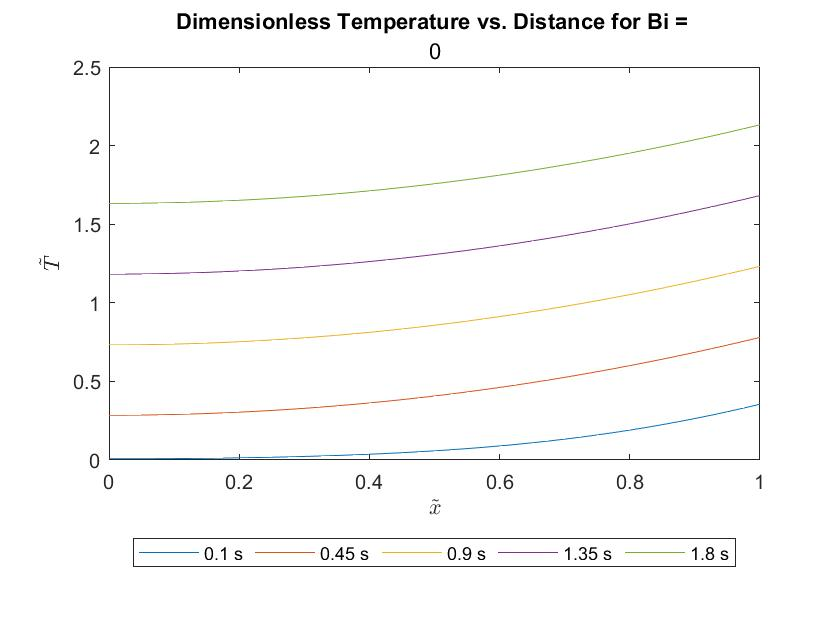
\includegraphics[width=.5\textwidth]{Bi0.jpg}
\caption{Water flowing through a pipe}
\end{figure}

\subsection{}
The first part of the problem asks for the heat transfer coefficient for the inner wall of the pipe to be plotted as a funtion of fluid velocity for Reynods number of 5,000 to 50,000.

The reynolds number for flow through a pipe is given as a function of the dydrodynamic diameter, the mean fluid velocity, density, and viscosity. 

\begin{equation}
\label{sample:equation}
   Re_D=\frac{\rho U_m D_i}{\mu}=\frac{U_m D_I}{\nu}
\end{equation}

For a circular pipe, the hydrodanamic diameter is the same as the inner diameter. Additionlly, for inconpressible fluids, the mean velocity remains constant. This allows the mean velocity to be calculated as a function of Reynolds number.

\begin{equation}
\label{sample:equation}
   U_m = \frac{Re_D \nu}{D_i}
\end{equation} 

The fully developed turbulent Nusselt number is a function of the Reynolds number, Prandtl Number, and friction. 

\begin{equation}
\label{sample:equation}
   Nu_{Dfd}=\frac{\left(\frac{f}{8}\right)(Re_D-1000)Pr}{1+12.7(Pr^{2/3}-1)\sqrt{\frac{f}{8}}}
\end{equation}

The heat transfer coefficient can be estimated as a function of the Nusselt number. This is a conservative estimation due to the Nusselt number being the averaged constant for the entire length of the pipe.

\begin{equation}
\label{sample:equation}
  h_i=frac{Nu_{Dfd}k_{H_2O}}{D_i}
\end{equation}

MATLAB functions with the properties of water were provided and can be found in Appendices B.1-B.6, using these, a program was written to olve for the velocity and heat transfer coffeicient for the given Reynolds numbers. The results were then plotted in figure 2, amd the code appears in attachment B.7.

\begin{figure}[hbt!]
\centering
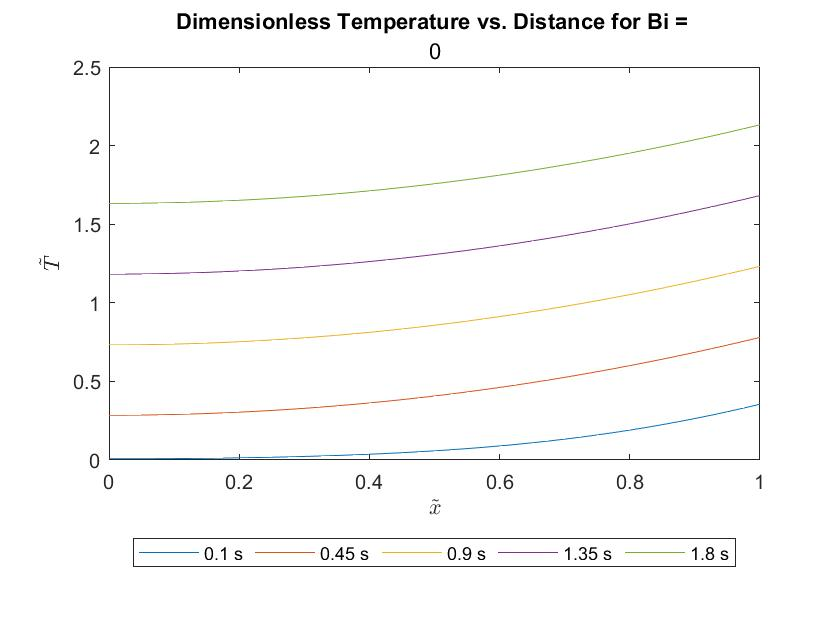
\includegraphics[width=.5\textwidth]{Bi0.jpg}
\caption{Interior convective heat transfer coeffecient vs Mean Velocity}
\end{figure}

\subsection{}
The next part of the problem asks for the exit temperatur of the pipe. This can be found using the differential energy balance.

\begin{equation}
\label{sample:equation}
  H_{in}+q''{out}=H_{in}+\frac{dH}{dx}dx
\end{equation}

\begin{equation}
\label{sample:equation}
  \dot{m}c_pT_m+\frac{T_\infty-T_m}{R'_tot}= \dot{m}c_pT_m+\dot{m}c_p\frac{dT}{dx}dx
\end{equation}

\begin{equation}
\label{sample:equation}
  \frac{T_\infty-T_m}{R'_tot}= \dot{m}c_p\frac{dT}{dx}dx
\end{equation}

Since $T_\infty$ and $R'_{tot}$ are estimated to be constant, rearranging and integrating yeilds the following equation for $T_{out}.

\begin{equation}
\label{sample:equation}
  T_{out}=t_\infty-(T_\infty-T_in)exp\left(-\frac{L}{R'_{tot}\dot{m}c_p}\right)
\end{equation}

$\frac{L}{R'{tot}}$ is equal to the total resistance $R{tot}$

\begin{equation}
\label{sample:equation}
  \frac{L}{R'_{tot}}=R_{tot}=\frac{1}{\bar{h_{i}}\pi D_{i}}+\frac{ln\left(\frac{D_{o}}{D_{i}}\right)}{2L\pi k_{steel}}+\frac{1}{\bar{h_o} \pi D_o L}
\end{equation}

Replacing $\frac{1}{R{tot}}$ with the variable UA gives


\begin{equation}
\label{sample:equation}
  T_{out}=t_\infty-(T_\infty-T_in)exp\left(-\frac{UA}{\dot{m}c_p}\right)
\end{equation}

\section{Problem 2}










\subsection{Crank-Nicolson}
The Crank Nicolson method is a second order in space and time, finite differencing method. It works by combining the forward Euler method at point n with the backward Euler method at point n+1. This combines the simplicity of the forward Euler with the stability of the backward Euler method, making it unconditionally stable. It can be expressed as follows:
\begin{equation}
\label{sample:equation}
\frac{\partial T}{\partial t}=\alpha \frac{1}{2}\left[\frac{\partial^2 T}{\partial x^2}^{t=j}+\frac{\partial^2 T}{\partial x^2}^{t=j+1}\right]
\end{equation}
Applying finite differencing to this yields:
\begin{equation}
\label{sample:equation}
\frac{T_i^{j+1}-T_i^j}{\Delta t}=\alpha \frac{1}{2}\left[\frac{T_{i+1}^j-2T_i^j+T_{i-1}^j}{\Delta x^2}+\frac{T_{i+1}^{j+1}-2T_i^{j+1}+T_{i-1}^{j+1}}{\Delta x^2}\right]
\end{equation}

Using the cell-dependent Fourier Number $Fo=\frac{\alpha \Delta t}{\Delta x^2}$ and rearranging, the following implicit/explicit expression for the temperature at position i and time j+1 can be reached:

\begin{equation}
\label{sample:equation}
  T_i^{j+1}-\frac{Fo}{2}\left[T_{i+1}^{j+1}-2T_i^{j+1}+T_{i-1}^{j+1}\right]=T_i^j+\frac{Fo}{2}\left[T_{i+1}^j-2T_i^j+T_{i-1}^j\right]
\end{equation}

This can be solved by expressing the previous equation as matrix function:

\begin{equation}
\label{sample:equation}
\bf{A} \cdot \bf{T}^{j+1}=\bf{B} \implies \bf{T}^{j+1} =\bf{A}^T \cdot \bf{B}
\end{equation}
Or: 
\begin{equation}
\label{sample:equation}
\begin{split}
\begin{bmatrix}
    &       &       & \cdots&       &       \\
-Fo &2(1+Fo)&-Fo    & 0     &\cdots &       \\
0   &-Fo    &2(1+Fo)&-Fo    & 0     &\cdots \\
    &       &       & \ddots&       &       \\
    &\cdots & 0     &-Fo    &2(1+Fo)&-Fo    \\
    &       &       & \cdots&       &   
\end{bmatrix} 
\cdot
\begin{bmatrix}
T_1^{j+1} \\
T_2^{j+1} \\
\\
\vdots\\
\\
T_N^{j+1} \\
\end{bmatrix} 
 \cr =
 \begin{bmatrix}
        &               &               & \cdots        &                   &           \\
FoT_1^j &2(1-Fo)T_2^j   &FoT_3^j        & 0             &\cdots             &           \\
0       &FoT_2^j        &2(1-Fo)T_3^j   &FoT_4^j        & 0                 &\cdots     \\
        &               &               & \ddots        &                   &           \\
        &\cdots         & 0             &Fo T_{N-2}^j   &2(1-Fo)T_{N-1}^j   &FoT_{N}^j  \\
        &               &               & \cdots        &                   &   
\end{bmatrix} 
\end{split}
\end{equation}

\subsection{Boundary Conditions} Now that the matrices have been built to solve for the interior nodes, the boundary conditions need to be handled. To do this, the energy balances at the first and last node will be calculated using the following:

\begin{equation}
\label{sample:equation}
   q_{1-}+q_{1+}=\frac{\rho c \Delta x}{2}\frac{\partial T_1}{\partial t}
\end{equation}

For the first node, heat transfer from the left is in the form of convection, $q_{1-}=-h(T_1-T_\infty)$, and from the right side is conduction with node 2, $q_{1+}=-k(T_1-T_2)/\Delta x$. The energy balance for node 1 can now be written.

\begin{equation}
\label{sample:equation}
h(T_\infty-T_1) + k\frac{(T_2-T_1)}{\Delta x}=\frac{\rho c \Delta x}{2}\frac{\partial T_1}{\partial t}
\end{equation}

Now the Crank Nicolson implicit/explicit method can be applied to the spatial differences and the equation discretized with respect to time.

\begin{equation}
\label{sample:equation}
\frac{h}{2}(T^j_\infty-T^j_1+T^{j+1}_\infty-T^{j+1}_1) + \frac{k}{2}\frac{(T^{j}_2-T^{j}_1+T^{j+1}_2-T^{j+1}_1)}{\Delta x}=\frac{\rho c \Delta x}{2}\frac{T_1^{j+1}-T^{j}_1}{\Delta t}
\end{equation}

\begin{equation}
\label{sample:equation}
\frac{h \Delta x}{k}(T^j_\infty-T^j_1+T^{j+1}_\infty-T^{j+1}_1) +(T^{j}_2-T^{j}_1+T^{j+1}_2-T^{j+1}_1)=\frac{\rho c \Delta x^2}{k \Delta t}(T_1^{j+1}-T^{j}_1)
\end{equation}

\begin{equation}
\label{sample:equation}
\frac{k \Delta t}{\rho c \Delta x^2}\frac{h \Delta x}{k}(T^{j+1}_\infty-T^{j+1}_1)
+\frac{k \Delta t}{\rho c \Delta x^2}(T_2^{j+1}-T_1^{j+1})-T_1^{j+1}
=
\frac{k \Delta t}{\rho c \Delta x^2}\frac{h \Delta x}{k}(T^{j}_1-T^{j}_\infty)
+\frac{k \Delta t}{\rho c \Delta x^2}(T_1^{j}-T_2^{j})-T_1^{j}
\end{equation}

Now the equation will be non-dimensionalized using $\tilde{q}=q/q_{ref}$, $\tilde{T}=T k/q_{ref}$, $\tilde{t}=\alpha t/L^2$, $\tilde{x}=x/L$, and $Bi_L=hL/k$. Additionally, $T_\infty$ is constant, so $T_\infty^j=T_infty^{j+1}=T_\infty$.

\begin{equation}
\label{sample:equation}
Fo Bi \Delta \tilde{x} \tilde{T}^{j+1}_1
+Fo (\tilde{T}_1^{j+1}-\tilde{T}_2^{j+1})-\tilde{T}_1^{j+1}
=
Fo Bi \Delta \tilde{x} (2\tilde{T}_\infty-\tilde{T}^{j}_1)
+Fo (\tilde{T}_2^{j}-\tilde{T}_1^{j})+\tilde{T}_1^{j}
\end{equation}

\begin{equation}
\label{sample:equation}
[Fo(Bi \Delta \tilde{x}+1)+1] (\tilde{T}^{j+1}_1)
-Fo \tilde{T}_2^{j+1}
=
Fo Bi \Delta \tilde{x} (2\tilde{T}_\infty-\tilde{T}^{j}_1)
+Fo (\tilde{T}_2^{j}-\tilde{T}_1^{j})+\tilde{T}_1^{j}
\end{equation}

This can now be used to create the first line of the matrix.
\\
The boundary condition at x=L is a conductive boundary where the heat flow varies with time. To find the energy balance, Equation 10 will be modified for node N.

\begin{equation}
\label{sample:equation}
   q_{N-}+q_{N+}=\frac{\rho c \Delta x}{2}\frac{\partial T_N}{\partial t}
\end{equation}

The heat flow from the left is $-k(T_N-T_{N-1})/\Delta x$, and the heat flow from the right is q(t).

\begin{equation}
\label{sample:equation}
   k\frac{(T_{N-1}-T_N)}{\Delta x}+q(t)=\frac{\rho c \Delta x}{2}\frac{\partial T_N}{\partial t}
\end{equation}

A non-dimensional equation can be derrived using the same process as for node 1.

\begin{equation}
\label{sample:equation}
   \frac{k}{2}\frac{(T^j_{N-1}-T^j_N+T^{j-1}_{N-1}-T^{j-1}_N)}{\Delta x}+\frac{1}{2}(q^j+q^{j-1})=\frac{\rho c \Delta x}{2}\frac{\partial T_N}{\partial t}
\end{equation}

\begin{equation}
\label{sample:equation}
   \frac{k \Delta t}{\rho c \Delta x^2}(T^j_{N-1}-T^j_N+T^{j-1}_{N-1}-T^{j-1}_N)+\frac{\Delta t}{\rho c \Delta x}(q^j+q^{j-1})=T^{j+1}_N-T^{j}_N
\end{equation}

\begin{equation}
\label{sample:equation}
   Fo (\tilde{T}^j_{N-1}-\tilde{T}^j_N+\tilde{T}^{j+1}_{N-1}-\tilde{T}^{j+1}_N)+Fo \Delta x (\tilde{q}^j+\tilde{q}^{j+1})=\tilde{T}^{j+1}_N-\tilde{T}^{j}_N
\end{equation}

\begin{equation}
\label{sample:equation}
   -Fo (\tilde{T}^{j+1}_{N-1}-\tilde{T}^{j+1}_N)+\tilde{T}^{j+1}_N=Fo (\tilde{T}^j_{N-1}-\tilde{T}^j_N)+\tilde{T}^{j}_N+Fo \Delta x (\tilde{q}^j+\tilde{q}^{j+1})
\end{equation}

\begin{equation}
\label{sample:equation}
   (Fo+1)\tilde{T}^{j+1}_N-Fo\tilde{T}^{j+1}_{N-1}=Fo (\tilde{T}^j_{N-1}-\tilde{T}^j_N)+\tilde{T}^{j}_N+Fo \Delta x (\tilde{q}^j+\tilde{q}^{j+1})
\end{equation}

\section{Results}
These changes were made to the two provided codes, which can be seen in Appendix A. It was then run with a Biot numbers of 0, 20, and 100 and plots of T vs. x were generated for t = 0.1, 0.45, 0.9, 1.35, and 1.8 s. These can be seen in Figures 1-3.
\\
\begin{figure}[hbt!]
\centering
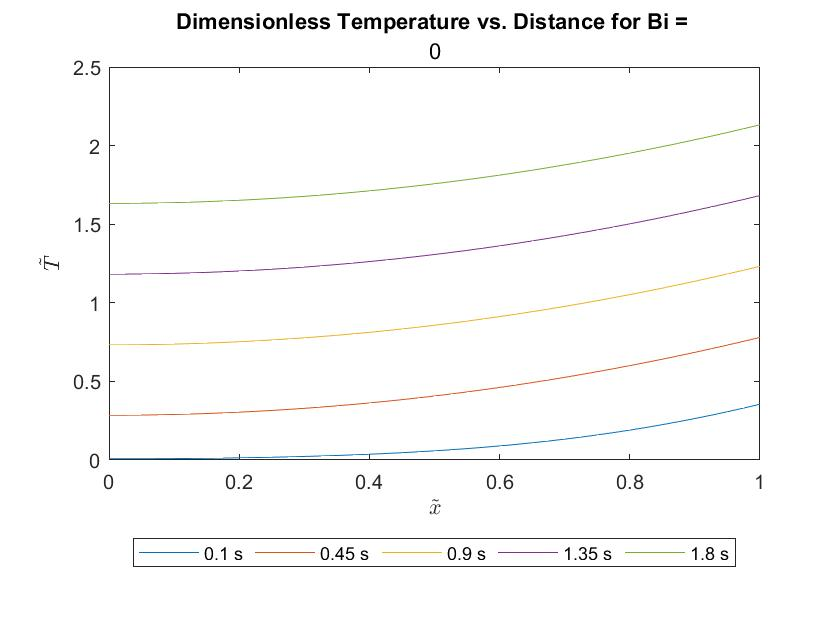
\includegraphics[width=.5\textwidth]{Bi0.jpg}
\caption{Results at $Bi_L$=0}
\end{figure}
\\
The results for the Biot number of 0 show that it behaves as if there is an adiabatic boundary at x = 0. Which could be predicted from understanding that convective transfer goes to 0 as the Biot number decreases, and from looking at equation 16. It can also be seen that early on, the left side stays at zero and starts to raise above zero and towards steady state once the diffusion reaches the left side and time advances.
\\
\begin{figure}[hbt!]
\centering
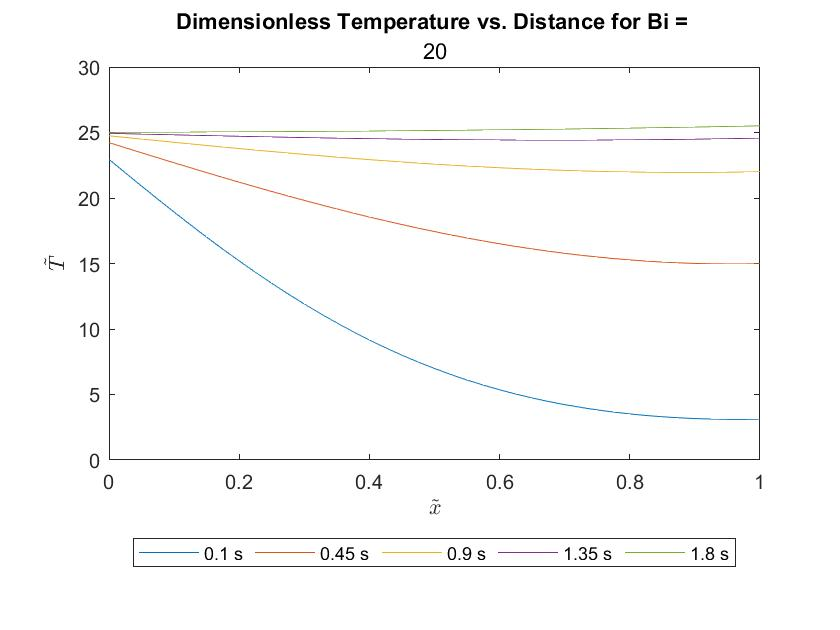
\includegraphics[width=.5\textwidth]{Bi20.jpg}
\caption{Results at $Bi_L$=20}
\end{figure}
\\
Looking at the results for a Biot number of 20, it can be seen that at the start most of the heat transfer is coming from the convective term and that the temperature at x=0 reaches the steady state temperature ($T_\infty$) quickly. However, the system does not reach steady state until 1.8 s. It can also be seen that the system balances out with the temperature at x=L slightly above that at x=0. This is to be expected since the boundary for x=L specifies a constant rate of heat flow into the system. This means that while at the start, the left boundary experiences convective heating and dominates the heat transfer rates into the system, after the system reaches steady state it becomes a convective cooling boundary to allow the release of the heat entering from the right boundary.
\begin{figure}[hbt!]
\centering
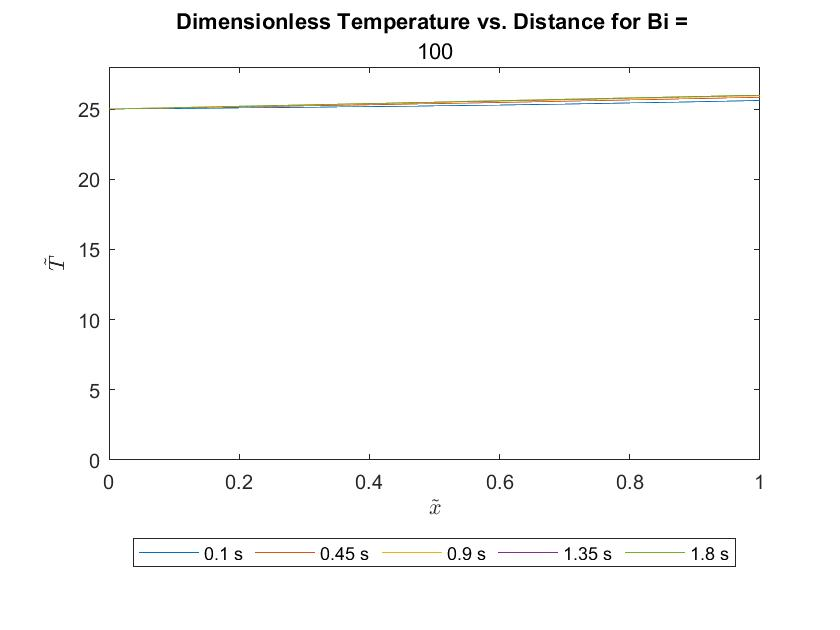
\includegraphics[width=.5\textwidth]{Bi100.jpg}
\caption{Results at $Bi_L$=100}
\end{figure}
\\
The results for the Biot number of 100 shows that the higher rate of heat transfer quickly brings the sytem up to temperature. It can also be seen that once the entire system has reached that of the free stream convective temperature on the left, the only heat into the system comes from the right boundary resulting in slower temperature increases.

\clearpage
\section*{Appendix A: MATLAB Code}

\begin{lstlisting}
close all
clear all
clc
m=0;
% script to run CN
% 
% space and time parameters
L=2;
nx = 40; % # segments
dt_tilde = 0.001; % time step (dimensionless)
x_tilde = [0:1/nx:1]; % x/L dimensionless

% reference parameters 
q_ref=10;
k=100;
T_ref=q_ref*L/k;
T_inf=5/T_ref;
T_tilde = zeros(nx+1,1);
t_final = 1.8; % given
time = [0 : dt_tilde : t_final ];
t_tilde = time/t_final;
q_tilde_0 = ones(length(time)); % given
nt = floor( t_final / dt_tilde );
for Bi=[0, 20, 100]
m=m+1;
% figure(1)
% plot( t_tilde, q_tilde_0,'LineWidth',3  );
% ax = gca;
% ax.FontSize = 30; 
% ylabel('Dimensionless heat flux','FontSize',30)
% xlabel('Dimensionless time','FontSize',30)
% title('Applied heat (dimensionless)')

T_tilde_save = zeros( length(t_tilde), nx+1 );
T_tilde_save(1, :) = T_tilde'; % save the initial condition
for j = 1 : length(t_tilde)-1
    T_tilde = fCrankNicolson2( nx, dt_tilde, T_tilde, Bi, T_inf, q_tilde_0(j), q_tilde_0(j+1));
    T_tilde_save(j+1, :) = T_tilde';
end

times=t_final/dt_tilde*[0.1, 0.45, 0.9, 1.35, 1.8]/1.8;
figure(m)
plot(x_tilde,T_tilde_save(times,:))
title('Dimensionless Temperature vs. Distance for Bi = ', Bi)
xlabel('$\tilde{x}$','Interpreter','latex')
ylabel('$\tilde{T}$','Interpreter','latex')
legend('0.1 s', '0.45 s', '0.9 s', '1.35 s', '1.8 s','Location','southoutside','Orientation','horizontal')
% figure(2)
% surf( x_tilde, t_tilde(1:nt-1), T_tilde_save(1:nt-1,:) );
% ax = gca;
% ax.FontSize = 30; 
% % xlabel('x_{tilde}','FontSize',30)
% % ylabel('Dimensionless time','FontSize',30)
% % zlabel('Dimensionless temp','FontSize',30)
% 
% figure(3)
% plot( t_tilde(1:nt-1), T_tilde_save( 1:nt-1, 1 ),'LineWidth',3  );
% ax = gca;
% ax.FontSize = 30; 
% % ylabel('Dimensionless temp','FontSize',30)
% % xlabel('Dimensionless time','FontSize',30)
end


function [T_tilde_new] = fCrankNicolson2(nx, dt_tilde, T_tilde_old, Bi, T_inf, q_tilde_j, q_tilde_jp1)
%
% Crank Nicolson routine to advance solution from t_j to t_jp1 (which is t_j+1)
%  X22B-0T0  q(t) = arbitrary function of time 
% constant properties
% nx = number of segments
%T_tilde_old = "old" temperature, dimensionless
% q_tilde_j = heat flux at the boundary at the current time
% q_tilde_jpq = heat flux at the boundary at the current time + dt_tilde
% dimensionless variables dt_tilde = alpha*dt/L^2 (time step)
%               computed  dx_tilde = L/nx = 1/nx
%                          T_tilde = T / (q_ref*L/k)
%                          q = q/q_ref
dx_tilde = 1/nx;
Fo = dt_tilde * nx^2;  % cell Fourier number, local dimensionless time = alpha*dt/dx^2, L = 1 nondimensionalized
Amat = zeros( nx+1, nx+1 );
RHS = zeros( nx+1, 1);
%

% fill the internal nodes first
for i = 2 : nx
    Amat(i,i-1) = -Fo/2;
    Amat(i,i) = 1 + Fo;
    Amat(i,i+1) = -Fo/2;
    RHS(i) = Fo/2 * (T_tilde_old(i-1)+T_tilde_old(i+1)) + (1-Fo) * T_tilde_old(i);
end

% boundary nodes
Amat(nx+1,nx) = -Fo;
Amat(nx+1, nx+1) = Fo + 1;
RHS(nx+1) = Fo*T_tilde_old(nx) + T_tilde_old(nx+1)*(1-Fo) + (q_tilde_j + q_tilde_jp1)*Fo/nx;

Amat(1,1) = (Fo*(Bi/nx+1)+1);
Amat(1,2) = -Fo;
RHS(1) = Fo*Bi/nx*(2*T_inf-T_tilde_old(1))+Fo*(T_tilde_old(2)-T_tilde_old(1))+T_tilde_old(1);
T_tilde_new = Amat \ RHS;  % "\" does something like forward elim/Back subst.
end




\end{lstlisting}
\end{document}